\documentclass[french]{article}
\usepackage[T1]{fontenc}
\usepackage[utf8]{inputenc}
\usepackage{lipsum}
\usepackage{lmodern}
\usepackage{geometry}
\usepackage{babel}
\usepackage{graphicx}
\usepackage{lastpage}
\usepackage{ragged2e}
\usepackage{enumitem}
\usepackage[normalem]{ulem}
\usepackage{hyperref} % pour \url{URL}
\usepackage{color} % pour \textcolor{color}{text}
\usepackage{listings} % pour afficher du code
\usepackage{longtable} % pour l'environnement longtable

% Grammaire EBNF
\usepackage{syntax}
\setlength{\grammarparsep}{5pt plus 1pt minus 1pt}
\setlength{\grammarindent}{11em}

% Diagramme de flux
\usepackage{tikz}
\usetikzlibrary{shapes,arrows}
\tikzstyle{decision} = [diamond, draw, fill=blue!20, text width=4.5em, text badly centered, node distance=3cm, inner sep=0pt]
\tikzstyle{block} = [rectangle, draw, fill=blue!20, text width=6em, text centered, rounded corners, minimum height=4em, node distance=3cm]
\tikzstyle{line} = [draw, -latex']
\tikzstyle{cloud} = [draw, ellipse,fill=red!20, node distance=3cm, minimum height=2em]

\geometry{
 	a4paper,
 	total={210mm,297mm},
 	left=20mm,
 	right=20mm,
 	top=20mm,
 	bottom=20mm,
}

\usepackage{fancyhdr}
\pagestyle{fancy}
\setlist[enumerate,1]{leftmargin=2cm}

% Entêtes
\lhead{Browne Champion Djomo Hardy Richoz Rochat}
\chead{}
\rhead{PRO}
\renewcommand{\headrulewidth}{0.4pt}
\renewcommand{\footrulewidth}{0.4pt}
	 
\begin{document}

	% Titre du document
	\title{GraphY} % ou un autre nom
	\author{Rapport\\ 
		Projet de semestre\\
		Browne Champion Djomo Hardy Richoz Rochat\\
		HEIG-VD}
	\date{\today} % date du jour
	\maketitle
	
	% Tables des matières
	\tableofcontents
	
	% Tables des figures
	\listoffigures
	
	% Pour tout le document
	\justify
	\normalsize
	
	\section{Cadre de développement} % Champion
		L'application est développée à l'aide du langage C++ et de la bibliothèque Qt \textcolor{red}{(insérer les versions utilisées ainsi que les compilateurs ?)}. Afin que le code source soit écrit dans le même style par tous les membres du groupe, nous avons décider d'utiliser le Coding Style de Qt qui correspond bien à nos besoins: \url{https://wiki.qt.io/Qt_Coding_Style}.
	
	\section{Normalisation du langage} % Champion
		Dans le cadre de l'application, l'utilisateur est amené à entrer des commandes lui permettant de créer et de modifier des graphes, tout autant que d'appeler des fonctions effectuant différents traitements (algorithmes, lecture depuis un fichier, ...). Il est donc nécessaire de définir une grammaire claire sur la syntaxe de ces commandes, ainsi que leur sémantique.
			
		\subsection{Analyse des types et des opérations} % Champion
			Premièrement, il faut définir les types disponibles dans le langage. Pour cela il est intéressant de partir des algorithmes de graphe et de voir les types de résultats que nous attendons en sortie, ainsi que les types de paramètres dont nous aurons besoin:
				
				\begin{itemize}
					\item Boolean: un graphe a-t-il un cycle? est-il eulérien? ...
					\item Number: poids d'un arc, indice d'un sommet, ...
					\begin{itemize}
						\item Integer: pour les index, ...
						\item Float: pour les poids, ...
					\end{itemize}
					\item String: label d'un sommet, nom d'une fonction, ...
					\item Array: liste d'arêtes, matrices (Floyd-Warshall), ...
					\item Graph: le graphe à proprement parler
					\begin{itemize}
						\item Vertex: un sommet, son indice, son poids, ...
						\item Edge: une arête/arc, son poids, ...
					\end{itemize}
				\end{itemize} 
				
			A présent que nous avons une idée des types disponibles, il faut définir leur domaine ainsi que les opérations disponibles et leur syntaxe. On fait le choix délibéré de se concentrer sur les opérations concernant les graphes, les opérations simples comme additionner deux nombres ou les comparaisons ne sont pas prévues. Cependant la base du langage doit permettre de les définir plus tard. 
			
				\begin{longtable}{lll}
					\textbf{\texttt{Boolean}}\\ \hline \hline
					Domaine & \multicolumn{2}{l}{\texttt{True} ou \texttt{False}}\\ 
					Opérations & Déclaration & \texttt{Boolean a = True;}\\
							   & Affectation & \texttt{a = False; a = f();}\\
							   & Lecture & \texttt{a; f(a); Boolean b = a;}\\ 
					\\
					\textbf{\texttt{Number}}\\ \hline \hline
					Domaine & \multicolumn{2}{l}{\texttt{Integer} et \texttt{Float}}\\ 
					\\
					\textbf{\texttt{Integer}}\\ \hline \hline
					Domaine & \multicolumn{2}{l}{Entier signé sur 32 bits}\\
					Opérations & Déclaration & \texttt{Integer a = -20;}\\
							   & Affectation & \texttt{a = 2; a = f();}\\
							   & Lecture & \texttt{a; f(a); Integer b = a;}\\ 
					\\
					\textbf{\texttt{Float}}\\ \hline \hline
					Domaine & \multicolumn{2}{l}{Nombre à virgule flottante sur 32 bits}\\
					Opérations & Déclaration & \texttt{Float a = -32.4;}\\
							   & Affectation & \texttt{a = 4.0; a = f();}\\
							   & Lecture & \texttt{a; f(a); Float b = a;}\\ 
					\\
					\textbf{\texttt{String}}\\ \hline \hline
					Domaine & \multicolumn{2}{l}{Ensemble de zéro ou plusieurs caractères ASCII}\\
					Opérations & Déclaration & \texttt{String a = "Hello";}\\
							   & Affectation & \texttt{a = "World"; a = f();}\\
							   & Lecture & \texttt{a; f(a); String b = a;}\\ 
					\\
					\textbf{\texttt{Array}}\\ \hline \hline
					Domaine & \multicolumn{2}{l}{Tableau dynamique hétérogène}\\
					Opérations & Déclaration & \texttt{Array a = [1.0, "Salut", 3];}\\
							   & Affectation & \texttt{a = [4, 5];}\\ 
							   & Lecture & \texttt{a; f(a); Array b = a;}\\
							   & Accès & \texttt{Integer c = a[1];}\\ 
					\\
					\textbf{\texttt{Vertex}}\\ \hline \hline
					Domaine & \multicolumn{2}{l}{Sommet avec des informations supplémentaires facultatives}\\
					Opérations & Déclaration & \texttt{Vertex a = (1); Vertex a2 = (2::3);}\\
							   & & \texttt{(id:label:weight:max\_capacity:min\_capacity)}\\
							   & Affectation & \texttt{a = (1:"Yverdon"); a = f();}\\
							   & Lecture & \texttt{a; f(a); Vertex b = a;}\\ 
					\\
					\textbf{\texttt{Edge}}\\ \hline \hline
					Domaine & \multicolumn{2}{l}{Arête/arc avec des informations supplémentaires facultatives}\\
					Opérations & Déclaration & \texttt{Edge a = (1--2); Edge a2 = (2<-3:5);}\\
							   & & \texttt{(connexion[id]:weight:label:max\_capacity:min\_capacity)}\\
							   & & \texttt{(arête: -- (tiret double) arcs: ->, <-)}\\
							   & Affectation & \texttt{a = (1->2::"A1"); a = f();}\\
							   & Lecture & \texttt{a; f(a); Vertex b = a;}\\ 
					\\
					\textbf{\texttt{Graph}}\\ \hline \hline
					Domaine & \multicolumn{2}{l}{Ensemble de sommets et d'arêtes/arcs (les parenthèses ne sont plus obligatoires)}\\
					Opérations & Déclaration & \texttt{Graph a = \{0, 1, 2:A, 1->2:3:::2]\};}\\
							   & & (si on ne veut pas écrire tous les sommets: \texttt{a = \{\#3, 0->1, 0->2\};})\\
							   & Affectation & \texttt{a = \{0, 1, 0--1\}; a = f();}\\
							   & Lecture & \texttt{a; f(a); Graph b = a;}\\
							   & Ajout/modification & \texttt{a += (1<-2:4)};\\
							   & Suppression & \texttt{a -= [(3), (1->2)];}\\
				\end{longtable}
				
			Ce tableau nous donne à présent une vue assez claire de nos besoins, cependant certaines opérations des types complexes (\texttt{Array, Vertex, Edge} et \texttt{Graph}) méritent d'être approfondies:
			
				\begin{itemize}
					\item \texttt{Array}: 
					\begin{itemize}
						\item Index de 0 à n-1
						\item Accès en dehors des bornes $\rightarrow$ Exception
					\end{itemize}
					\item \texttt{Vertex}:
					\begin{itemize}
						\item Seul le premier paramètre (\texttt{id[Integer]}) est obligatoire, et il ne doit pas être négatif
						\item Les valeurs par défaut sont \texttt{label[String]="", weight[Number]=0, max\_capacity[Number]=min\_capacity, min\_capacity[Number]=0}
					\end{itemize}
					\item \texttt{Edge}: 
					\begin{itemize}
						\item Seul le premier paramètre (\texttt{connexion}) est obligatoire
						\item Le paramètre \texttt{id[Integer]} doit être positif ou nul et sa valeur par défaut est 0
						\item Les valeurs par défaut sont \texttt{weight[Number]=0, label[String]="", max\_capacity[Number]=min\_capacity, min\_capacity[Number]=0}
						\item L'\texttt{id} est un identifiant "local" à la \texttt{connexion}
					\end{itemize}
					\item \texttt{Graph}: 
					\begin{itemize}
						\item La création d'un graphe vide est permis (\texttt{Graph g = \{\};})
						\item Le raccourci d'écriture pour le nombre de sommet (\texttt{\#3}) doit se trouver au début
						\item Pour que le \texttt{Vertex} d'\texttt{id n} soit créé, il faut que tous les \texttt{id} de \texttt{0} à \texttt{n-1} existent déjà, sinon $\rightarrow$ Exception 
						\item Dans le cas d'arêtes/arcs multiples, par exemple \texttt{\{\#2, 0->1, 0->1\}}, le paramètre \texttt{id} du second \texttt{Edge} est incrémenté $\rightarrow$ \texttt{0->1[0]} et \texttt{0->1[1]}
						\item Pour qu'un \texttt{Edge} soit créé, il est nécessaire que les deux \texttt{Vertex} soit déjà créés, sinon $\rightarrow$ Exception
						\item Ajouts / modifications:
						\begin{itemize}
							\item Les types acceptés en opérande de droite sont \texttt{Vertex, Edge} ou un \texttt{Array} de ces deux types
							\item Pour les \texttt{Vertex}, si l'\texttt{id} existe déjà dans le graphe, c'est une modification, sinon c'est un ajout
							\item Pour les \texttt{Edge}, si la \texttt{connexion} existe déjà dans le graphe mais que l'\texttt{id} est omis, alors c'est un ajout, sinon c'est une modification (sauf si l'\texttt{id} n'existe pas, dans ce cas c'est un ajout)
							\item La modification est accumulative, par exemple si on fait \texttt{Graph g = \{0:"Yverdon"\}; g += (0::2);}, alors le \texttt{Vertex} résultant est \texttt{(0:"Yverdon":2)}
						\end{itemize}
						\item Suppressions:
						\begin{itemize}
							\item Les types acceptés en opérande de droite sont \texttt{Vertex, Edge} ou un \texttt{Array} de ces deux types
							\item S'il n'y a rien à supprimer, alors il ne se passe rien (pas d'exception)
							\item La suppression d'un \texttt{Vertex} entraine la suppression des \texttt{Edge} associés
							\item Pour les \texttt{Edge}, si l'\texttt{id} est omis, alors toutes les \texttt{connexion} sont supprimées
						\end{itemize}
					\end{itemize}
				\end{itemize}
				
			Notons que les erreurs sont gérées au travers d'exceptions.\\
			
			Maintenant que les types des variables et leurs opérations de base sont définis, on veut pouvoir effectuer d'autres traitements sur ces variables (ajouter une nouvelle opération ou appliquer un algorithme). Cela va se faire via des fonctions prédéfinies (la définition de fonction n'est pas prévue).\\
			
			Prototype d'une fonction: \texttt{R f(T1, T2, ...);} avec \texttt{R} le type de retour, \texttt{f} le nom de la fonction et \texttt{Tn} le type du paramètre en position \texttt{n}.\\
			
			Appel d'une fonction: \texttt{Graph a = dijkstra(g, 1);} ou \texttt{g = removeAllPonderation(g);}.\\
			
			Le passage des paramètres se fait par copie (ou référence constante) et la correspondance est par position.
			
		\subsection{Grammaire EBNF} % Champion
			L'analyse étant finie, on peut à présent développer les règles de production EBNF du langage. On part des règles de haut niveau pour descendre dans la hiérarchie (inspiration: \url{http://www.fit.vutbr.cz/study/courses/APR/public/ebnf.html}).
			
			\subsubsection{Point de départ (entrée utilisateur)}
				\begin{grammar}
					<start> ::= <statement> \{ <statement> \}
				\end{grammar}
			
			\subsubsection{Déclarations (statements)}
				\begin{grammar}
					<statement> ::= ( <function-call> | <declaration> | <assignment> ) \lit{;}
					
					<function-call> ::= <identifier> <parameter-list>
					
					<declaration> ::= <type> <identifier> \lit{=} <parameter>
					
					<assignment> ::= <variable> \lit{=} <parameter>
					
					<parameter-list> ::= \lit{(} <parameter> \{ \lit{,} <parameter> \} \lit{)}
					
					<parameter> ::= <constant> | <indexed-array> | <function-call>
				\end{grammar}
			
			\subsubsection{Expressions et opérations}
				\begin{grammar}
					<indexed-array> ::= <variable> \lit{[} <digit-sequence> \lit{]}
				\end{grammar}
			
			\subsubsection{Types de variable et d'enregistrement}
				\begin{grammar}
					<type> ::= <simple-type> | <complex-type>
					
					<simple-type> ::= \lit{Boolean} | \lit{Number} | \lit{Integer} | \lit{Float} | \lit{String}
					
					<complex-type> ::= \lit{Array} | \lit{Graph} | \lit{Vertex} | \lit{Edge}
					
					<array-record> ::= \lit{[} <constant> \{ \lit{,} <constant> \} \lit{]}
					
					<constant> ::= <simple-constant> | <complex-constant>
					
					<complex-constant> ::= <array-record> | <graph-record> | <edge-record> | <vertex-record>
					
					<graph-record> ::= \lit{\{} <graph-info> \{ \lit{,} <graph-info> \} \lit{\}}
					
					<edge-record> ::= \lit{(} <edge-info> \lit{)}
					
					<vertex-record> ::= \lit{(} <vertex-info> \lit{)}
					
					<graph-info> ::= <vertex-info> | <edge-info>
					
					<edge-info> ::= <connexion> 
					\alt <connexion> \lit{:} <number>
					\alt <connexion> \lit{:} [ <number> ] \lit{:} <string>
					\alt <connexion> \lit{:} [ <number> ] \lit{:} [ <string> ] \lit{:} <number>
					\alt <connexion> \lit{:} [ <number> ] \lit{:} [ <string> ] \lit{:} [ <number> ] \lit{:} <number>
					
					<vertex-info> ::= <id> 
					\alt <id> \lit{:} <string>
					\alt <id> \lit{:} [ <string> ] \lit{:} <number>
					\alt <id> \lit{:} [ <string> ] \lit{:} [ <number> ] \lit{:} <number>
					\alt <id> \lit{:} [ <string> ] \lit{:} [ <number> ] \lit{:} [ <number> ] \lit{:} <number>
					
					<connexion> ::= <id> ( \lit{\textendash\textemdash} | \lit{\textemdash\textgreater} | \lit{\textless\textemdash} ) <id>
					
					<id> ::= <digit-sequence>
				\end{grammar}
		
			\subsubsection{Identifiants et définitions de bas niveau}
				\begin{grammar}
					<simple-constant> ::= <sign> <variable> | <number> | <boolean> | <string>
					
					<variable> ::= <identifier>
					
					<identifier> ::= <letter> \{ <letter> | <digit> | \lit{\_} \}
					
					<string> ::= \lit{"\""} \{ <letter> | \lit{ } \} \lit{"\""}
					
					<letter> ::= ? all lower and upper case letters ? 
					
					<boolean> ::= \lit{True} | \lit{False}
					
					<number> ::= <integer-number> | <real-number>
					
					<real-number> ::= [ <sign> ] <digit-sequence> \lit{.} <digit-sequence>
					
					<integer-number> ::= [ <sign> ] <digit-sequence>
					
					<digit-sequence> ::= <digit> \{ <digit> \}
					
					<sign> ::= \lit{+} | \lit{-} 
					
					<digit> ::= ? all digits from 0 to 9 ? 
				\end{grammar}
			
		\subsection{Conception de l'interpréteur}
			Le langage est à présent clairement définit, cependant il faut encore concevoir l'interpréteur qui permettra de vraiment l'utiliser:
			
			\begin{figure}[h!]
				\centering
				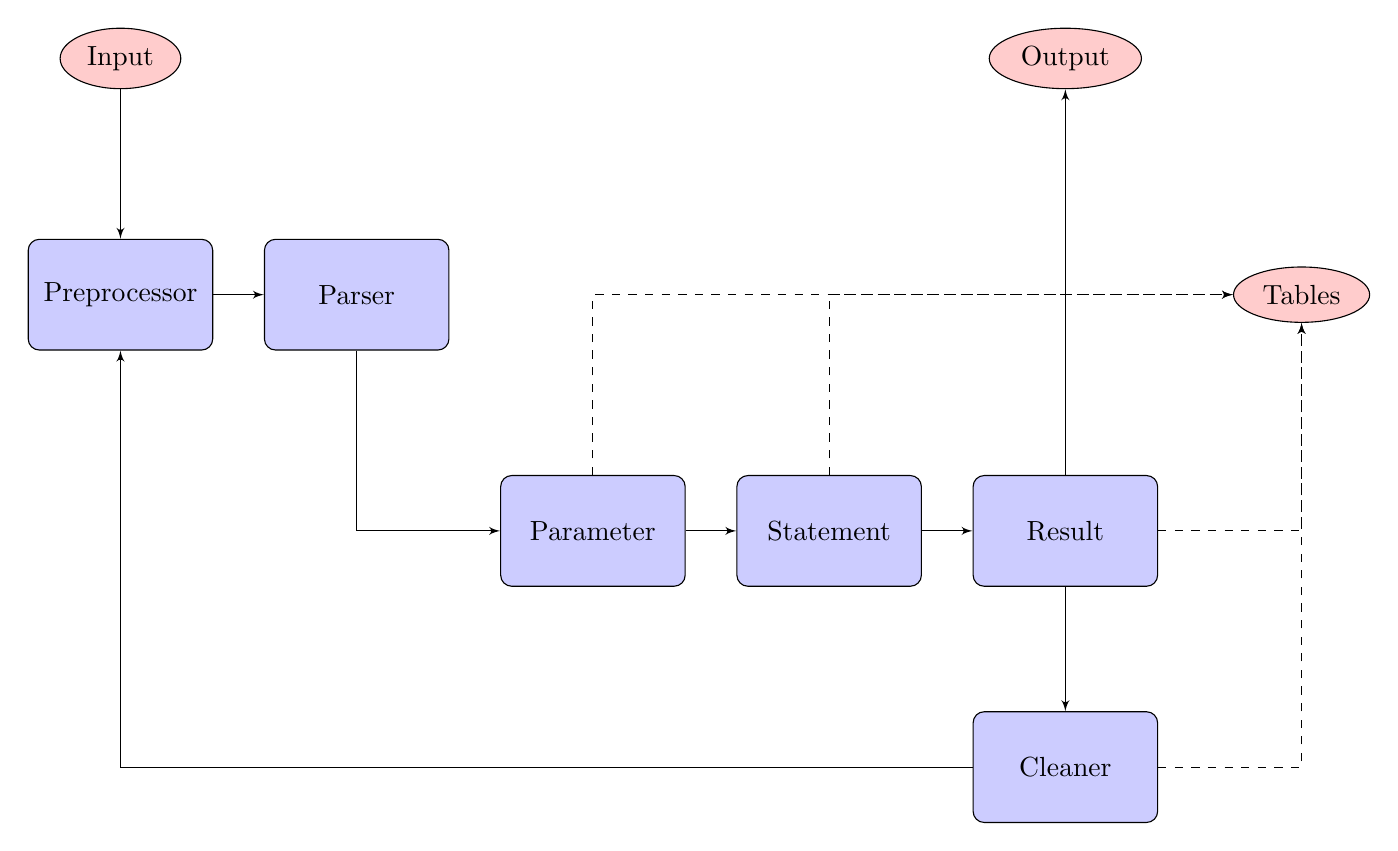
\begin{tikzpicture}[node distance = 1cm, auto]
					\node [block] (preprocessor) {Preprocessor};
					\node [block, right of=preprocessor] (parser) {Parser};
					\node [block, below of=parser, right of=parser] (parameters) {Parameter};
					\node [block, right of=parameters] (statement) {Statement};
					\node [block, right of=statement] (return) {Result};
					\node [block, below of=return] (clean) {Cleaner};
					\node [cloud, right of=return, above of=return] (table) {Tables};
					\node [cloud, above of=preprocessor] (input) {Input};
					\node [cloud, above of=parser, above of=return] (output) {Output};
					\path [line] (input) -- (preprocessor);
					\path [line] (preprocessor) -- (parser);
					\path [line] (parser) |- (parameters);
					\path [line] (parameters) -- (statement);
					\path [line] (statement) -- (return);
					\path [line] (return) -- (output);
					\path [line] (return) -- (clean);
					\path [line] (clean) -| (preprocessor);
					\path [line,dashed] (parameters) |- (table);
					\path [line,dashed] (statement) |- (table);
					\path [line,dashed] (return) -| (table);
					\path [line,dashed] (clean) -| (table);
				\end{tikzpicture}
				\caption{Flux des données dans l'interpréteur}
			\end{figure}
			
			bla bla TODO
		
		\section{Annexes}
			\subsection{Références}
				...
				
\end{document}
